\documentclass[laboratorio]{guia}

\def \practnum {6} 
\def \practica {Circuito RLC: resonancia en serie y en paralelo}

\def \materia {Laboratorio de F\'\i sica II para Qu\'\i micos}
\def \periodo {2\sptext{o} cuatrimestre de 2016}
\def \profesor {Diana Skigin}
\def \website {http://materias.df.uba.ar/f2qa2016c2}
 
\usepackage{graphics}
\usepackage{amsmath}
\usepackage{amsfonts}
\usepackage{graphicx}
\usepackage{float}
\usepackage{wrapfig}
\usepackage{subfigure}
\usepackage{bm}
\usepackage{grffile}
\usepackage{color}
\usepackage{framed}
\usepackage[utf8]{inputenc}
\usepackage[T1]{fontenc}
\usepackage{lmodern} 
% definicion del entorno 'sabermas'
\makeatletter
\definecolor{shadecolor}{rgb}{0.89,0.91,0.94}
\newenvironment{sabermas}[1]{%
\vfill
\begin{shaded}
  \begin{center}
  {\textsection{Para saber m\'as}}
  \end{center}
  #1
\sf } 
{%
\end{shaded}%
}
\makeatother

\renewcommand{\vec}[1]{\ensuremath{\mathbf{#1}}}




\hyphenation{ coe-fi-cien-tes coe-fi-cien-te au-to-va-lor
              au-to-va-lo-res co-rres-pon-der pro-ble-ma 
              cual-quie-ra po-la-ri-za-cio-nes }

\graphicspath{{./Guia_06_Circuito_RLC/}}

\begin{document} 
\objetivo{Estudiar los comportamientos de un circuito RC en dos reg\'\i menes de operaci\'on 
    distintos: (a) transitorio y (b) estacionario. Para el transitorio, se
    propone estudiar los procesos de carga y descarga de un capacitor en un
    circuito RC. Caracterizar ambos determinando qu\'e tipo de evoluc\'on
    temporal presentan, y midiendo los tiempos caracter\'\i sticos asociados
    a cada uno de ellos. Para el estacionario, se busca determinar la respuesta
    del circuito al excitarlo con una se\~nal peri\'odica, variando la
    frecuencia de trabajo del sistema.
    \tematicas{Circuitos de corrientes variables en el tiempo, RLC, resonancia.}} 
\maketitle

\section{Desarrollo de la experiencia}

Considere el circuito RC mostrado en la Figura \ref{fig:circuitoRC}, en el
cual el capacitor se encuentra completamente descargado inicialmente y la
llave S, abierta. Al cerrarse esta \'ultima, la diferencia de potencial
$V$ impuesta por la fuente genera una corriente $I$ en el circuito. Esta 
corriente tendr\'a el efecto de llevar cargas de signo opuesto a las caras 
del capacitor. Resulta intuitivo que esta corriente no ser\'a constante en el tiempo; 
en particular esperamos que la misma se anule cuando el capacitor se haya
cargado. 


\begin{figure}[t!]
    \centering
    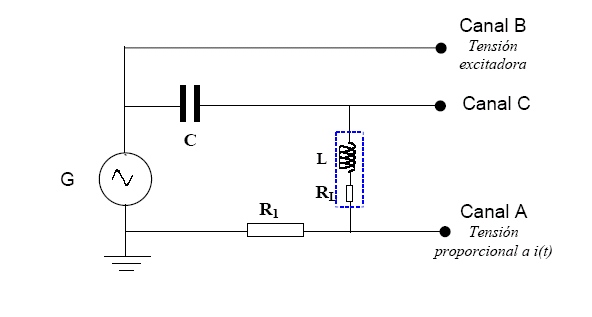
\includegraphics[width=8.5cm]{LG06--000.png}
    \caption{}
    \label{fig:1}
\end{figure}

\begin{figure}[t!]
    \centering
    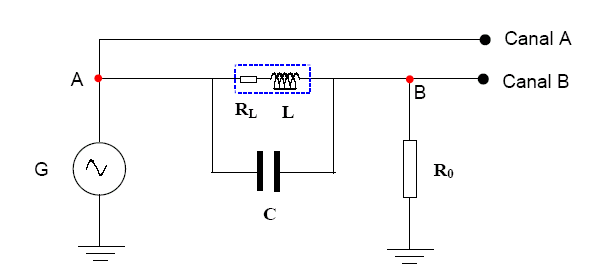
\includegraphics[width=8.5cm]{LG06--001.png}
    \caption{}
    \label{fig:2}
\end{figure}


\nocite{Alonso1998,Purcell1988,Reitz1996,Trelles1984,Reitz1996}
\bibliographystyle{unsrt} 
\bibliography{Bibliografia}

%  \bibliographystyle{unsrt} \bibliography{biblio}

\end{document}
